\renewcommand{\teacherTag}{QUESTION 8 \textbullet\ 35 MARKS}
\chapter{The Fourier Transform: Impulses, Pulses and Applications}

%------------------------------------------------------------------ 8(a)
\begin{qcard}{Q8(a)}{Transform of shifted impulses}{5 + 5}
(i) Using the sifting property of the impulse, find the Fourier transform of $x(t)=\delta(t-a)$.\\
(ii) The signal $p_k(t)$ consists of $k$ equally spaced unit impulses at $t=1,2,\dots,k$:
\[p_k(t)=\delta(t-1)+\delta(t-2)+\dots+\delta(t-k)=\sum_{m=1}^k\delta(t-m).\]
Using (i), the additivity of the Fourier transform and the sum of a geometric series, show that $P_k(j\omega)=\dfrac{e^{-j\omega}\big(1-e^{-jk\omega}\big)}{1-e^{-j\omega}}$.
\end{qcard}
\begin{solution}
\step{(i)} Sifting: $\int f(t)\delta(t-a)\dd t=f(a)$. With $f(t)=e^{-j\omega t}$:
\[X(j\omega)=\int_{-\infty}^{\infty}\delta(t-a)\,e^{-j\omega t}\dd t=e^{-j\omega a}.\]
Magnitude $1$ at all frequencies (an impulse contains every frequency equally); phase $-\omega a$, a straight line whose slope is the delay.

\step{(ii) Step 1 --- additivity.} Transform term by term using (i) with $a=m$:
\[P_k(j\omega)=\sum_{m=1}^{k}e^{-j\omega m}.\]
\step{Step 2 --- geometric series.} Let $q=e^{-j\omega}$ (assume $q\ne1$, i.e.\ $\omega\ne2\pi n$). The sum is $q+q^2+\dots+q^k$, first term $q$, ratio $q$, $k$ terms:
\[P_k(j\omega)=q\,\frac{1-q^k}{1-q}=\boxed{\frac{e^{-j\omega}\big(1-e^{-jk\omega}\big)}{1-e^{-j\omega}}}\]
At $\omega=2\pi n$ every term equals 1 and $P_k=k$ (the limit of the formula).

\step{Step 3 --- a useful closed form.} Factor half-angles: $1-e^{-jk\omega}=e^{-jk\omega/2}\,2j\sin\frac{k\omega}2$ and $1-e^{-j\omega}=e^{-j\omega/2}\,2j\sin\frac\omega2$:
\[P_k(j\omega)=e^{-j\omega(k+1)/2}\,\frac{\sin(k\omega/2)}{\sin(\omega/2)} .\]
The phase is linear (centre of the train at $t=\frac{k+1}2$) and the magnitude is the periodic ``Dirichlet'' pattern with peaks $k$ at $\omega=2\pi n$.
\begin{center}
\begin{tikzpicture}\begin{axis}[width=12cm,height=4.4cm,axis lines=middle,xlabel={$\omega$},title={$\abs{P_k(j\omega)}=\abs{\sin(k\omega/2)/\sin(\omega/2)}$ for $k=5$},xmin=-7.5,xmax=7.9,ymin=0,ymax=5.8,xtick={-6.2832,-3.1416,0,3.1416,6.2832},xticklabels={$-2\pi$,$-\pi$,$0$,$\pi$,$2\pi$},ytick={1,5},yticklabels={$1$,$k=5$},ticklabel style={font=\scriptsize},label style={font=\scriptsize},title style={font=\scriptsize},samples=600]
\addplot[very thick,navy,domain=-7.5:7.5]{abs(sin(deg(2.5*x))/max(abs(sin(deg(x/2))),0.0005))*(abs(sin(deg(x/2)))>0.0005)+5*(abs(sin(deg(x/2)))<=0.0005)};
\end{axis}\end{tikzpicture}
\end{center}
\ans{(i) $\delta(t-a)\pair e^{-j\omega a}$. (ii) $P_k(j\omega)=\sum_{m=1}^ke^{-j\omega m}=\dfrac{e^{-j\omega}(1-e^{-jk\omega})}{1-e^{-j\omega}}=e^{-j\omega(k+1)/2}\dfrac{\sin(k\omega/2)}{\sin(\omega/2)}$.}
\end{solution}

%------------------------------------------------------------------ 8(b)
\begin{qcard}{Q8(b)}{A stepped pulse from rectangular pulses}{10}
Consider $x(t)=1$ for $1<t<2$, $2$ for $2<t<3$, $1$ for $3<t<4$, and $0$ otherwise. Given the pair
\[r_T(t)=\begin{cases}1,&\abs t<\frac T2\\0,&\text{otherwise}\end{cases}\qquad\pair\qquad R_T(j\omega)=\frac{2\sin(\omega T/2)}{\omega},\]
find $X(j\omega)$ without directly evaluating the Fourier transform integral.
\end{qcard}
\begin{solution}
\step{Step 1 --- Build $x$ from rectangles.} The signal is symmetric about $t=2.5$. It is a wide pulse of height 1 on $(1,4)$ plus a narrow pulse of height 1 on $(2,3)$:
\[x(t)=r_3(t-2.5)+r_1(t-2.5).\]
(Check: on $(2,3)$ both are 1, total 2; on $(1,2)$ and $(3,4)$ only the wide one, total 1.)
\begin{center}
\begin{tikzpicture}\begin{axis}[width=5.4cm,height=3.8cm,axis lines=middle,xlabel={$t$},title={$x(t)$},xmin=0,xmax=5,ymin=0,ymax=2.5,xtick={1,2,3,4},ytick={1,2},ticklabel style={font=\scriptsize},label style={font=\scriptsize},title style={font=\scriptsize}]
\addplot[very thick,navy]coordinates{(0,0)(1,0)(1,1)(2,1)(2,2)(3,2)(3,1)(4,1)(4,0)(5,0)};\end{axis}\end{tikzpicture}
\raisebox{12mm}{$=$}
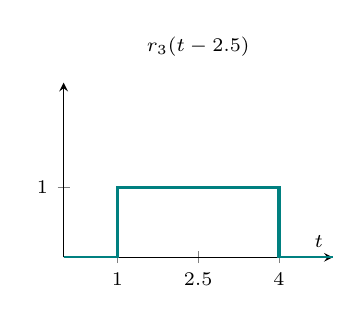
\begin{tikzpicture}\begin{axis}[width=5.0cm,height=3.8cm,axis lines=middle,xlabel={$t$},title={$r_3(t-2.5)$},xmin=0,xmax=5,ymin=0,ymax=2.5,xtick={1,2.5,4},ytick={1},ticklabel style={font=\scriptsize},label style={font=\scriptsize},title style={font=\scriptsize}]
\addplot[very thick,teal]coordinates{(0,0)(1,0)(1,1)(4,1)(4,0)(5,0)};\end{axis}\end{tikzpicture}
\raisebox{12mm}{$+$}
\begin{tikzpicture}\begin{axis}[width=5.0cm,height=3.8cm,axis lines=middle,xlabel={$t$},title={$r_1(t-2.5)$},xmin=0,xmax=5,ymin=0,ymax=2.5,xtick={2,3},ytick={1},ticklabel style={font=\scriptsize},label style={font=\scriptsize},title style={font=\scriptsize}]
\addplot[very thick,coral]coordinates{(0,0)(2,0)(2,1)(3,1)(3,0)(5,0)};\end{axis}\end{tikzpicture}
\end{center}
\step{Step 2 --- Transform each piece.} From the given pair, $r_3\pair\dfrac{2\sin(3\omega/2)}{\omega}$ and $r_1\pair\dfrac{2\sin(\omega/2)}{\omega}$. A shift by $2.5$ multiplies by $e^{-j2.5\omega}$ (part (a)(i): shifting is convolution with $\delta(t-2.5)$).

\step{Step 3 --- Linearity.}
\[\boxed{X(j\omega)=e^{-j2.5\omega}\,\frac{2\big[\sin(1.5\,\omega)+\sin(0.5\,\omega)\big]}{\omega}}\]
Using $\sin A+\sin B=2\sin\frac{A+B}2\cos\frac{A-B}2$ (with $A=1.5\omega$, $B=0.5\omega$), an equivalent form is
\[X(j\omega)=e^{-j2.5\omega}\,\frac{4\sin\omega\,\cos(\omega/2)}{\omega}.\]

\step{Check.} $X(0)=\lim\frac{2(1.5\omega+0.5\omega)}{\omega}=4=\int x(t)\dd t=1+2+1$ \checkmark. The magnitude is real and even (the pulse is symmetric about its centre); the shift contributes only the linear phase $-2.5\omega$.
\begin{center}
\begin{tikzpicture}\begin{axis}[width=12cm,height=4.4cm,axis lines=middle,xlabel={$\omega$},title={$\abs{X(j\omega)}=\abs{2[\sin1.5\omega+\sin0.5\omega]/\omega}$},xmin=-13,xmax=13.6,ymin=0,ymax=4.6,xtick={-12.566,-6.2832,-3.1416,0,3.1416,6.2832,12.566},xticklabels={$-4\pi$,$-2\pi$,$-\pi$,$0$,$\pi$,$2\pi$,$4\pi$},ytick={4},ticklabel style={font=\scriptsize},label style={font=\scriptsize},title style={font=\scriptsize},samples=500]
\addplot[very thick,navy,domain=-13:13]{abs(2*(sin(deg(1.5*x))+sin(deg(0.5*x)))/(x+0.00001))};
\end{axis}\end{tikzpicture}
\end{center}
\ans{$X(j\omega)=e^{-j2.5\omega}\Big[\dfrac{2\sin(3\omega/2)}{\omega}+\dfrac{2\sin(\omega/2)}{\omega}\Big]=e^{-j2.5\omega}\dfrac{4\sin\omega\cos(\omega/2)}{\omega}$, with $X(0)=4$.}
\end{solution}

%------------------------------------------------------------------ 8(c)
\begin{qcard}{Q8(c)}{Three applications of the Fourier transform}{5 + 5 + 5}
Briefly describe how the Fourier transform can be used in each scenario. (i) An image of a metal surface contains cracks and object boundaries; we need an image in which these edges are emphasised. (ii) A large image must be transmitted through a slow link; we have to compress it while retaining its main visual appearance. (iii) A music recording is corrupted by persistent noise at frequencies above the useful range of the music; we have to reduce this noise without disrupting the music.
\end{qcard}
\begin{solution}
\begin{keyidea}Smooth regions $=$ low frequencies; sharp changes (edges, fine detail, hiss) $=$ high frequencies. Filtering in the Fourier domain is just multiplying the spectrum by a mask $H$ and transforming back, since $y=x*h\iff Y=XH$.\end{keyidea}

\step{(i) Edge enhancement --- high-pass filtering.} Take the 2-D Fourier transform $X(u,v)$ of the image. Cracks and boundaries are abrupt changes in brightness, so their energy sits at \emph{high spatial frequencies}, while the smooth background is near $(0,0)$. Multiply by a high-pass mask $H(u,v)$ that suppresses frequencies near the origin and keeps (or boosts) the outer region, then take the inverse transform. The result shows the edges bright on a dark background; adding it back to the original (``high-boost''/sharpening) gives an image with emphasised edges. (Equivalently, differentiation $\leftrightarrow$ multiplication by $j\omega$, which grows with frequency.)

\step{(ii) Compression --- keep the strong low-frequency coefficients.} For natural images most of the energy is concentrated in a small number of low-frequency coefficients (energy compaction; Parseval says energy is preserved, so we can see where it is). Transform the image (in practice blockwise, as with the DCT in JPEG), \emph{quantise} the coefficients and \emph{discard} the many small high-frequency ones, then send only the remaining few (entropy-coded). The receiver inverse-transforms them: the main shapes and shading survive; only fine detail is lost, which the eye hardly notices.

\step{(iii) Noise removal --- low-pass filtering.} Compute the spectrum of the recording; the music occupies $\abs f\le f_{\max}$ and the persistent noise lies above it. Apply a low-pass filter with cutoff just above $f_{\max}$ (multiply the spectrum by $H(f)=1$ for $\abs f\le f_{\max}$, $\approx0$ above, with a smooth transition and linear phase so the waveform is not distorted), then inverse transform (or use the equivalent FIR filter $h=\F^{-1}\{H\}$ in real time). The music band is untouched while the out-of-band noise is removed.
\begin{center}
\begin{tikzpicture}[x=0.55cm,y=1.1cm,>=Stealth]
\draw[->](-0.3,0)--(13.6,0)node[right,font=\scriptsize]{$\abs f$};
\fill[navy!25](0,0)--(0,0.95)to[out=-10,in=170](6,0.5)--(6.6,0)--cycle;\node[font=\tiny,navy]at(2.6,1.15){music};
\fill[crimson!30](7.4,0)rectangle(13,0.35);\node[font=\tiny,crimson]at(10.2,0.55){persistent noise};
\draw[very thick,teal](0,1.3)--(6.8,1.3)to[out=0,in=180](7.4,0.02)--(13,0.02);\node[font=\tiny,teal,anchor=south]at(3.4,1.32){low-pass $H(f)$};
\draw[dashed](7,0)--(7,1.45)node[above,font=\tiny]{cutoff $\approx f_{\max}$};
\end{tikzpicture}
\end{center}
\ans{(i) High-pass filter the 2-D spectrum (edges are high-frequency) and add back to sharpen; (ii) transform, keep and quantise the few large low-frequency coefficients, drop the small high-frequency ones (JPEG-style); (iii) low-pass filter with cutoff just above the music band.}
\end{solution}
